\documentclass{article}
\usepackage[utf8]{inputenc}
\usepackage{enumitem}
\usepackage{float}
\usepackage{siunitx}
\sisetup{group-separator={'}, group-digits=integer}
\usepackage{graphicx}
\graphicspath{ {./img/} }

\title{Bloom Filter}
\author{Timothy Grützner, Jonas Möller, Nathanael Weber }
\date{\today}

\begin{document}

    \maketitle
    \newpage


    \section{Idee}
    Die Idee des Bloom Filters ist relativ simpel. Es wird geprüft, ob in einem vorgegebenen Set ein Element vorhanden ist oder nicht. Anhand eines Beispiels kann der Bloom Filter anschaulich erklärt werden:\\ Es ist ein leeres Set (z.B. Array) vorgegeben mit einer bestimmten Anzahl an Indizes. In unserem Fall sind es die Indizes 0 bis 29, sprich 30 Elemente in diesem Set. Jeder Index, der kein Element besitzt, tritt als 0 Bit auf.
    Damit ein Element zu diesem Set hinzugefügt wird (z.B. das Wort "dist") muss dieses vorher mehrfach mit einem Hash gehasht werden. Für unseren Fall nehmen wir das Hashverfahren "murmur" mit jeweils einem Seed. Dieser Seed ändert sich bei jedem Hashingdurchlauf, sodass bei jedem Hashingvorgang ein unterschiedlicher Hash für dasselbe Wort generiert wird. \\
    Bei jedem Hashing bekommen wir eine Nummer. Diese wird Modulo der Länge des Filters gerechnet, damit wir bei zu grossen Hashwerten keine Zahlen verlieren. Anschliessend wird an dem Index im Filter des berechneten Wertes das Bit 1 gesetzt. \\
    Jenachdem, wie gross man die Fehlerwahrscheinlichkeit haben will, braucht man einen unterschiedlich grossen Filter sowie eine unterschiedliche Anzahl an Hashingvorgängen. \\
    Nehmen wir nun an, dass wir eine Anzahl von 2 Hashingvorgängen haben. Dann könnte es beim Hashen des Wortes "dist" die beiden Hashwerte $1$ sowie $23$ geben, sodass wir wir an Position \verb|Set[1]| sowie \verb|Set[23]| das Bit auf $1$ setzen. Diese Schritte werden bei jedem Hinzufügen eines Elements analog durchgeführt, nur dass idealerweise andere Hashwerte generiert werden.\\\\
    Die notwendigen Grössen des Filters werden anhand der Anzahl erwarteter Elemente $n$ und der gewünschten Fehlerwahrscheinlichkeit $\varepsilon$ berechnet.\\\\
    $m$ = Geeignete Filtergrösse\\
    $n$ = Anzahl erwartender Elemente\\
    $k$ = Optimale Anzahl Hash Funktionen\\
    \noindent $\varepsilon = $ Fehlerwahrscheinlichkeit
    \\

    \noindent Formel für die geeignete Filtergrösse:
    $$
    m=-\frac{n \ln \varepsilon}{(\ln 2)^{2}}
    $$
    \\
    Formel für die optimale Anzahl Hash Funktionen:
    $$
    k=\frac{m}{n} \ln 2
    $$

    \vspace{.5cm}

    \noindent Um nun zu Testen ob ein Element enthalten ist, wird das gesuchte Elemente durch das gleiche bzw. die gleichen Hashvorgänge gelassen und geprüft, ob sich jeweils an Position dieses Hashwerts im Set eine Bit 1 befindet. Falls ja, dann kann das Wort sich im Set befinden. \\
    Der Bloom Filter kann einer der folgenden Aussagen machen:
    \begin{itemize}
        \item Befindet sich ein Element definitiv nicht im Set
        \item Das Element könnte sich im Set befinden
    \end{itemize}

    \noindent Die Genauigkeit des Filters sprich die Wahrscheinlichkeit eines "false positive" kann bei der Instanziierung angegeben werden. Sie berechnet sich anhand der Anzahl Hash Funktionen $k$ und der Filtergrösse $m$.

    $$
    P=\left(1-\left[1-\frac{1}{m}\right]^{k n}\right)^{k}
    $$
    \\
    \noindent Geeignete und oft genutzte Hashingverfahren sind z.B. HashMix, murmur und auch fnv. Es kann mit unterschiedlichen Seeds gearbeitet werden, damit nur ein Hashingverfahren angewendetet werden muss, dass folglich mit unterschiedlichen Seeds unterschiedliche Hashwerte für dieselbe Eingabe ausgibt.

    \subsection{Vorteile}
    Der Hauptvorteil des Bloom-Filters ist offensichtlich: \\
    Die enorme Geschwindigkeit bei grossen Datenmengen. Kaum eine Datenstruktur arbeitet so schnell wie der Bloom Filter, mit so wenig Speicherverbrauch. Die Datenstruktur, die dem Bloom-Filter zu Grunde liegt, ist betreffend dem Speicher sehr vorteilhaft, dies dank des einfachen Bitvektors als Datenstruktur. Die Grösse des Filters $m$ ist abhängig von der tolerierten Wahrscheinlichkeit eines "false positives" $\varepsilon$ und der Anzahl Elemente im Filter $n$. Dabei wächst $m$ nur sehr langsam, wie an der bereits erwähnten Formel zu erkennen ist.

    \subsection{Nachteile}
    \begin{itemize}[leftmargin=*]
        \item Der Filter arbeitet niemals 100\% genau! Je kleiner die Wahrscheinlichkeit $\varepsilon$ sein soll, desto grösser ist der Datenverbrauch. Eine Wahrscheinlichkeit von exakt $0$ kann niemals erreicht werden.
        \item Das Löschen von Elementen ist nicht möglich. Es ist grundsätzlich möglich, dass mehrere Elemente den gleichen erzeugten Hash haben und somit würden auch andere Elemente gelöscht werden bei Löschung eines Bits aus dem Array.
        \item Nicht alle Hashingverfahren eignen sich für den Einsatz im Bloomfilter, sondern nur schnelle (dies bedeutet keine kryptographisch sicheren). Unter die kryptographischen fallen z.B. die oft genutzten Hashingverfahren SHA und MD5. Diese Hashingverfahren sind aufgrund Ihrer längeren Laufzeit für den Bloomfilter nicht geeignet, da der Bloomfilter vorallem performant und schnell sein muss.
    \end{itemize}


    \section{Beispiel}
    Ein anschauliches Beispiel in der Praxis ist dort zu finden, wo grosse Datenmengen schnell verarbeitet werden müssen. Wenn zum Beispiel eine Person eine neue Google-Email-Adresse anlegen möchte, dann muss die gesamte Datenbanken innerhalb kürzester Zeit überprüft werden, um dem Benutzer mit minimaler Verzögerung anzugeben, ob die Email-Adresse bereits vorhanden ist oder nicht. Dies bewerkstelligt der Bloom-Filter mit der Aussage: "Das Element kann sich im Set befinden". Mit dieser Aussage kann diese Email-Adresse nicht verwendet werden, dies wird dem Benutzer fast Live angezeigt. Somit muss sich der Benutzer eine andere Email-Adresse auswählen. \\
    In diesem Beispiel ist es auch nicht so schlimm, wenn die erst gewählte Mail-Adresse eigentlich trotzdem noch nicht vorhanden ist.


    \section{Unser Programm}
    Wir haben unser Programm in Java geschrieben und das Collection Interface implementiert, damit man damit wie bei einer normalen Java Collection arbeiten kann. Natürlich werfen die "remove" Methoden aber eine Fehlermeldung, da dies bei einem einfachen Bloom Filter nicht möglich ist. \\
    Dies könnte aber auf verschiedene Wege hinzugefügt werden, bei jeder Möglichkeit ist der Bloom Filter aber anschliessend entweder weniger schnell oder benutzt mehr Speicher.

    \subsection{Testen der Fehler-Wahrscheinlichkeit}
    Wir benutzen die Anzahl der Wörter im \texttt{words.txt} sowie die vom Benutzer gewünschte Fehler-Wahrscheinlichkeit, um den Filter zu initialisieren. \\
    Anschliessend fügen wir jedes Wort dem Filter hinzu. Wir überprüfen kurz jedes Wort, um sicherzustellen, dass es auch tatsächlich im Filter enthalten ist. Ist dies nicht der Fall, terminieren wir, da eine wichtige Invariante des Filters verletzt wäre.\\
    Um die Fehler-Wahrscheinlichkeit nun zu testen, machen wir auf jedem Wort im \texttt{words.txt} ein Cäsar mit dem Parameter 2 um ein neues Wort zu erhalten. Nun prüfen wir für jedes dieser Wörter (nachdem wir alle rausgeworfen haben, welche trotzdem bereits im \texttt{words.txt} existieren), ob der Filter uns ein false-positive gibt oder richtig erkennt dass das Wort nicht im Filter ist. \\
    Am Schluss teilen wir dann die Anzahl an false-positives durch die Anzahl an Wörtern im Filter, was uns die Fehler-Wahrscheinlichkeit ergibt.


    \newpage

    \subsection{Resultat der Tests}
    In unseren Tests waren wir jeweils sehr Nahe an der Fehler-Wahrscheinlichkeit, welche wir via Input am Anfang des Programms eingestellt haben. Dies war für uns sehr erfreulich.
    \begin{sloppypar}
        \begin{table}[h]
            \caption{Szenarien}
            \begin{tabular}{*4{S[table-format=6.0]}}
                \hline\hline
                \textbf{Gewünschtes $\varepsilon$} & \textbf{Filter Grösse} & \textbf{Anzahl "false positives"} & \textbf{Tatsächliches $\varepsilon$} \\ [0.5ex]
                \hline
                0.2                                & 194658                 & 12254                             & 0.2108                               \\
                0.05                               & 362328                 & 2961                              & 0.0509                               \\
                0.01                               & 556987                 & 626                               & 0.0107                               \\
                0.001                              & 835481                 & 60                                & 0.001033                             \\
                0.0001                             & 1113975                & 4                                 & 0.000069 \\ [1ex]
                \hline
            \end{tabular}
        \end{table}
    \end{sloppypar}
    \begin{figure}[h]
        \centering
        \caption{Output for $\varepsilon$ = 0.001}
        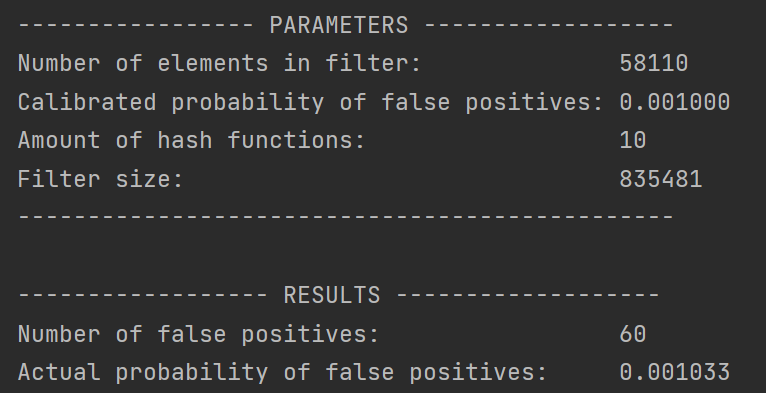
\includegraphics{programoutput}
    \end{figure}

\end{document}
